\chapter{Experimental results}
\section[Introduction]{Introduction \hfill \small \normalfont\textit{by Alessandro Motta}}

In our challenging journey of setting up our agent for the ring against other agents we always had to try different combinations of the functions we created. These are the reinforcement learning method, normalizing the state, the different features and the game settings, such how many coins, crates and steps there are in each game. While playing around with all the different functions we created we wanted a way to measure how good our agent was learning. To safe some samples that indicated how our agent was learning we created a folder named "Histories" that contained a \texttt{.pt} file with the different stats of the game. Such as the number of coins collected, the number of invalid moves etc. This helped us to  keep track of what settings lead us to which results. The next step was to write code to help us monitor these results in a clear and structured way. This file is called \texttt{monitoring.py}. To help explain our thought process we will divide the section of experimental result in 3 different parts in which we will also explain what interesting observations we made and what changes we: 
\begin{itemize}
\item[(1)] Coin collector (collect coins in an open field)
\item[(2)] Crate agent (set bombs to collect coins)
\item[(3)] Simulation study: n-step Sarsa vs trace-decay
\end{itemize}

\section[Coin collecting agent ]{Coin collecting agent  \hfill \small \normalfont\textit{by Alessandro Motta}}
\subsection{Exploiting symmetries}
The first mission of our agent was to collect coins in an open field without any crates. For this mission we started exploiting the symmetries and had as features: the coin map with look around, the wall map with look around and the coins in quartal; while using an epsilon-greedy policy. We set the end of a game at 3000 steps and multiplied x3 the number of coins that spawned in a game. For the last setting we wrote a function that multiplies the coins. After implementing this function we observed that it was possible for the game to spawned more than a coin at the same position, so we decided to change that. In our first monitoring we wanned to be sure that training while exploiting two spatial symmetries led to a quicker learning process then not exploiting any.
\begin{center}
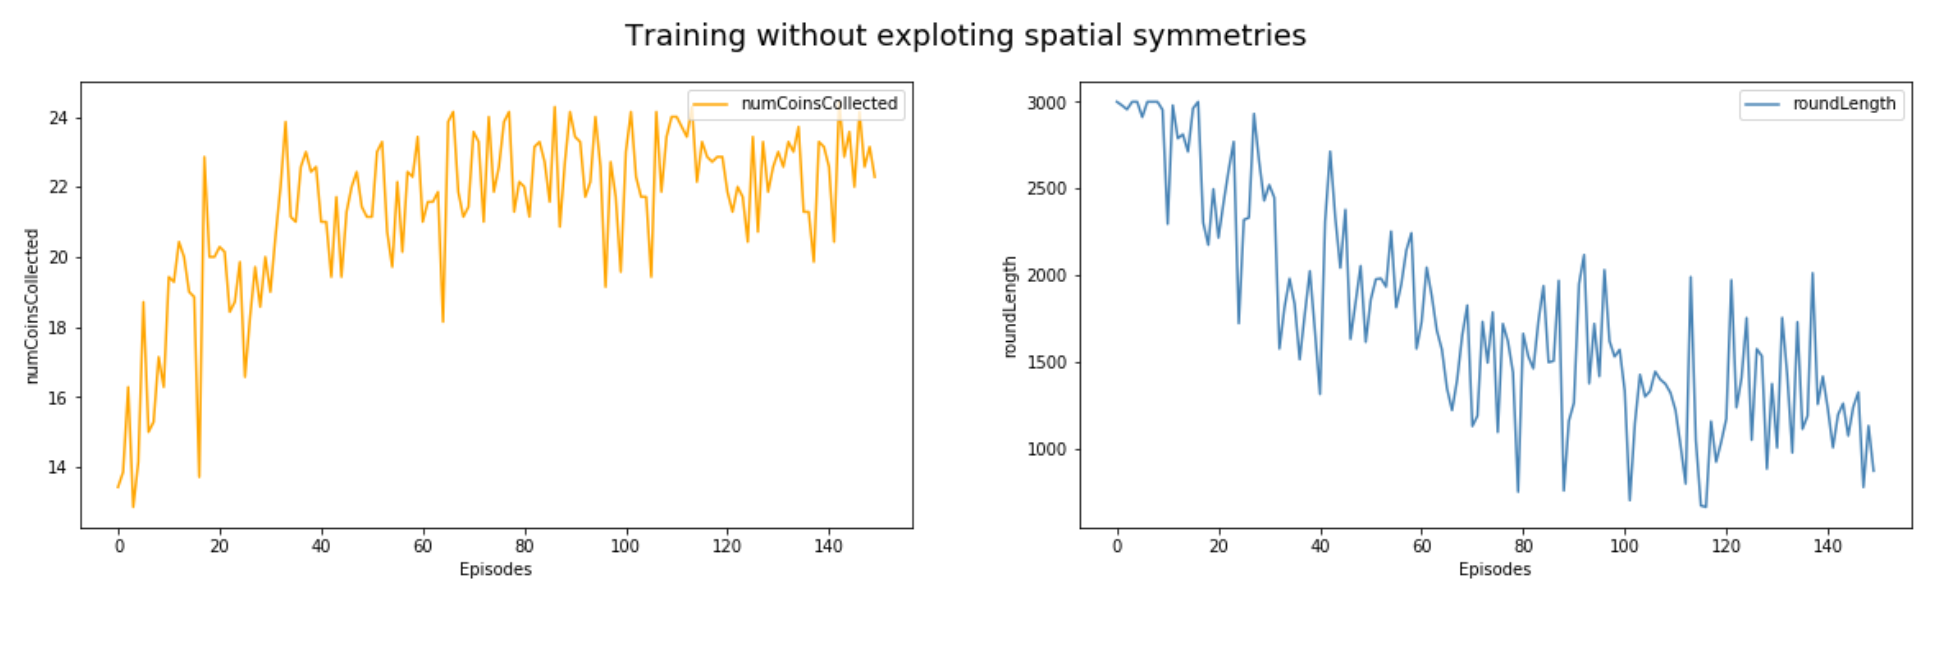
\includegraphics[scale=0.22]{graphics/plot01.png}
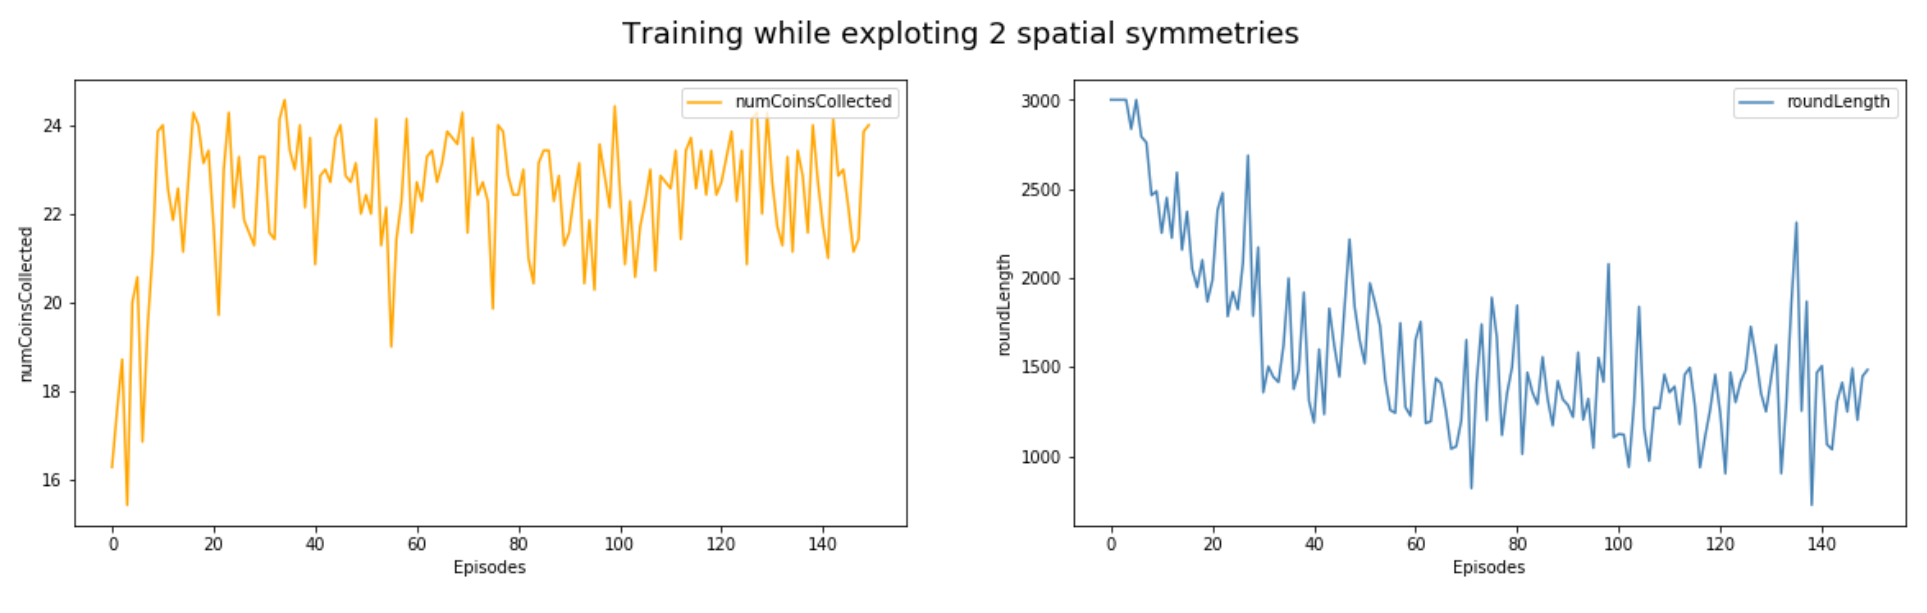
\includegraphics[scale=0.22]{graphics/plot02.png}
\end{center}
As we could observe a better learnig curve we decided to exploit the third spetial symmetry. The diagonal spetial symmetry. 
\begin{center}
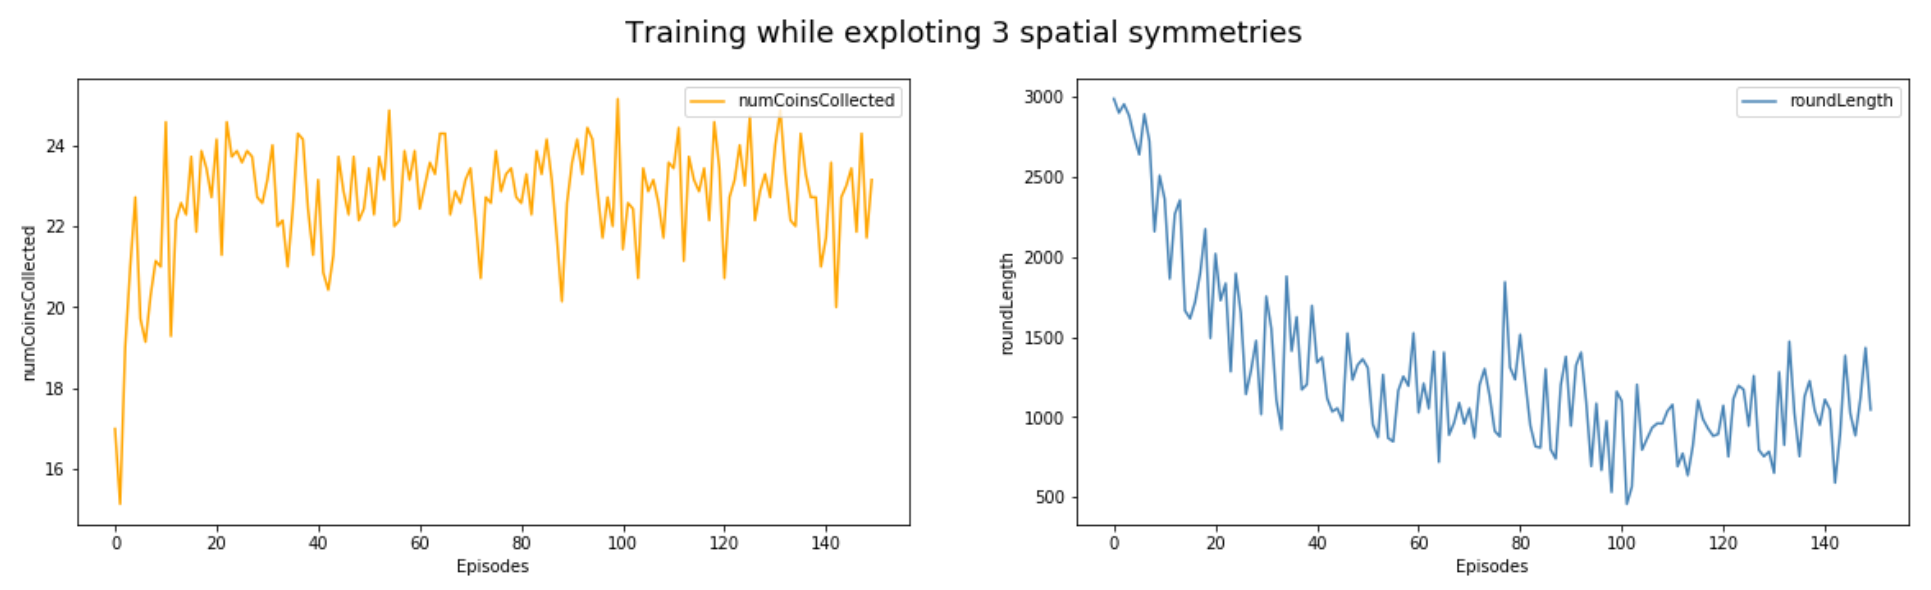
\includegraphics[scale=0.22]{graphics/plot03.png}
\end{center}

\subsection{The quartal feature problem}
As of this point we started noticed a big problem: Mostly when in playing mode our agent started to get stuck and repeat the same two moves after each step, going up and down or left and right for the rest of the game. This is because in playing mode we set a low epsilon so that he would do less random moves and just select the "good ones" with the idea that while playing he did not need to explore. We discovered that the agent got stuck because when there were only a few coins left he could not decide to which quartal he should go. The only way he could get out of repeating these moves over and over was after by performing a random action and get out of this state. Since in training mode there was a higher chance of doing a random move (bigger epsilon) he did not get stuck as often as in training mode. We tried to fix this bug by rewriting the coins in quartal feature but the problem persisted. So we decided to use a higher epsilon also when in playing mode. This helped to get out of this bug-state quicker, but we still had one problem, we needed a lot of moves to collect all the coins. We came upwith two different solutions for this problem: 1)Implementing a softmax policy. A softmax will also help us in our next task, since when our agent sets a bomb he cannot allow himself to do at random all actions with the same probability. 2)Implementing a feature that describes where the next nearest coin is.

\subsection{Shortest path feature}
After implementing the shortes path feature we managed to fix the bug and got really good results as we can see in the next graph.
\begin{center}
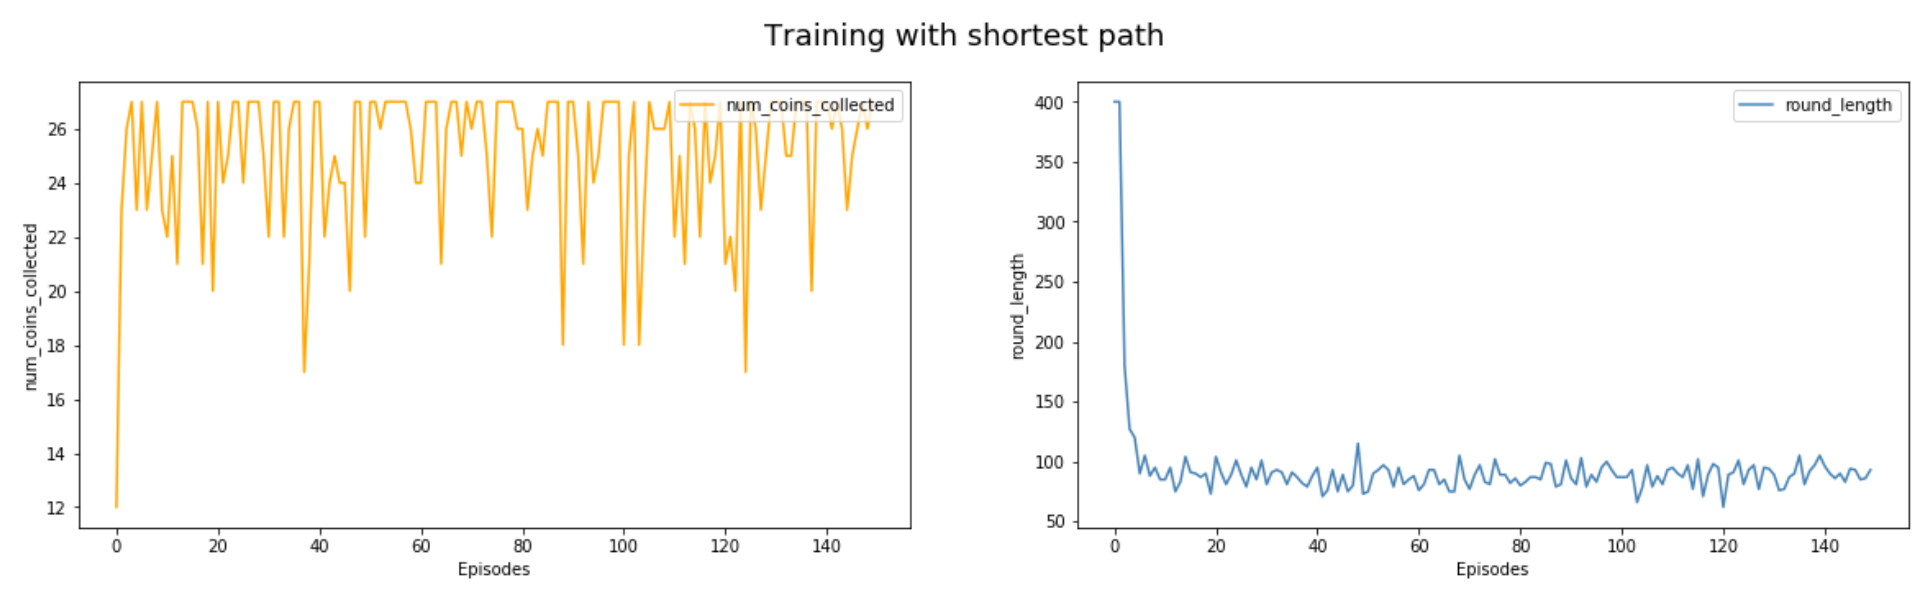
\includegraphics[scale=0.22]{graphics/plot04.png}
\end{center}

\section[Crate agent]{Crate agent  \hfill \small \normalfont\textit{by Alessandro Motta}}
\subsection{Setup}
In this section the task of our agent was to destroy crates in order to collect the coins around the map. Therefore we needed to implement new features and had to change our monitoring in order to see how many bombs were dropped, how many crates were destroyed and other helpful things that we started implementing along the way. A big challenge was to keep track of all the trainings with all the different game, methods and feature settings. Since we tried to train with as much combinations as possible. To help us train as much combinations as possible we wrote a shell script (train.sh) so that with one execution of the code we could train multiple agents for certain number of episodes. Afterwards we wrote a \texttt{simulation\_study.py} to make our agent train during the night with different combinations.

\subsection{Agent behavior in relation to rewards}
We tried to fine tune our reward system but did not really come to the results we were hoping for. During all our test we had some really inconsistent results. We observed that really small changes in the reward system could make really big differences in the behavior of the agent. The most challenging thing was trying to make the number of crates that were being destroyed during the game converge. As we can see in the following graph the behavior of the bot was really polarized. We understood while training that no matter what rewards we gave him he could only learn two different behaviors.
\begin{enumerate}
\item Dropping a bomb everytime he could was good. We gave him a small reward for dropping bombs, a big one for collecting coins, destroying crates and a negative reward for dying. This led that directly when spawning he started dropping bombs. We can see this in the graph when he drops 80 bombs per round (we trained for a round length of 400 steps and he can drop a bomb every 5 rounds, $400 \setminus5 = 80$). Sadly sometimes the crate layout is made so that if you release a bomb at the beginning of the game you have no escape and you die in the fifth round.
\end{enumerate}
\begin{center}
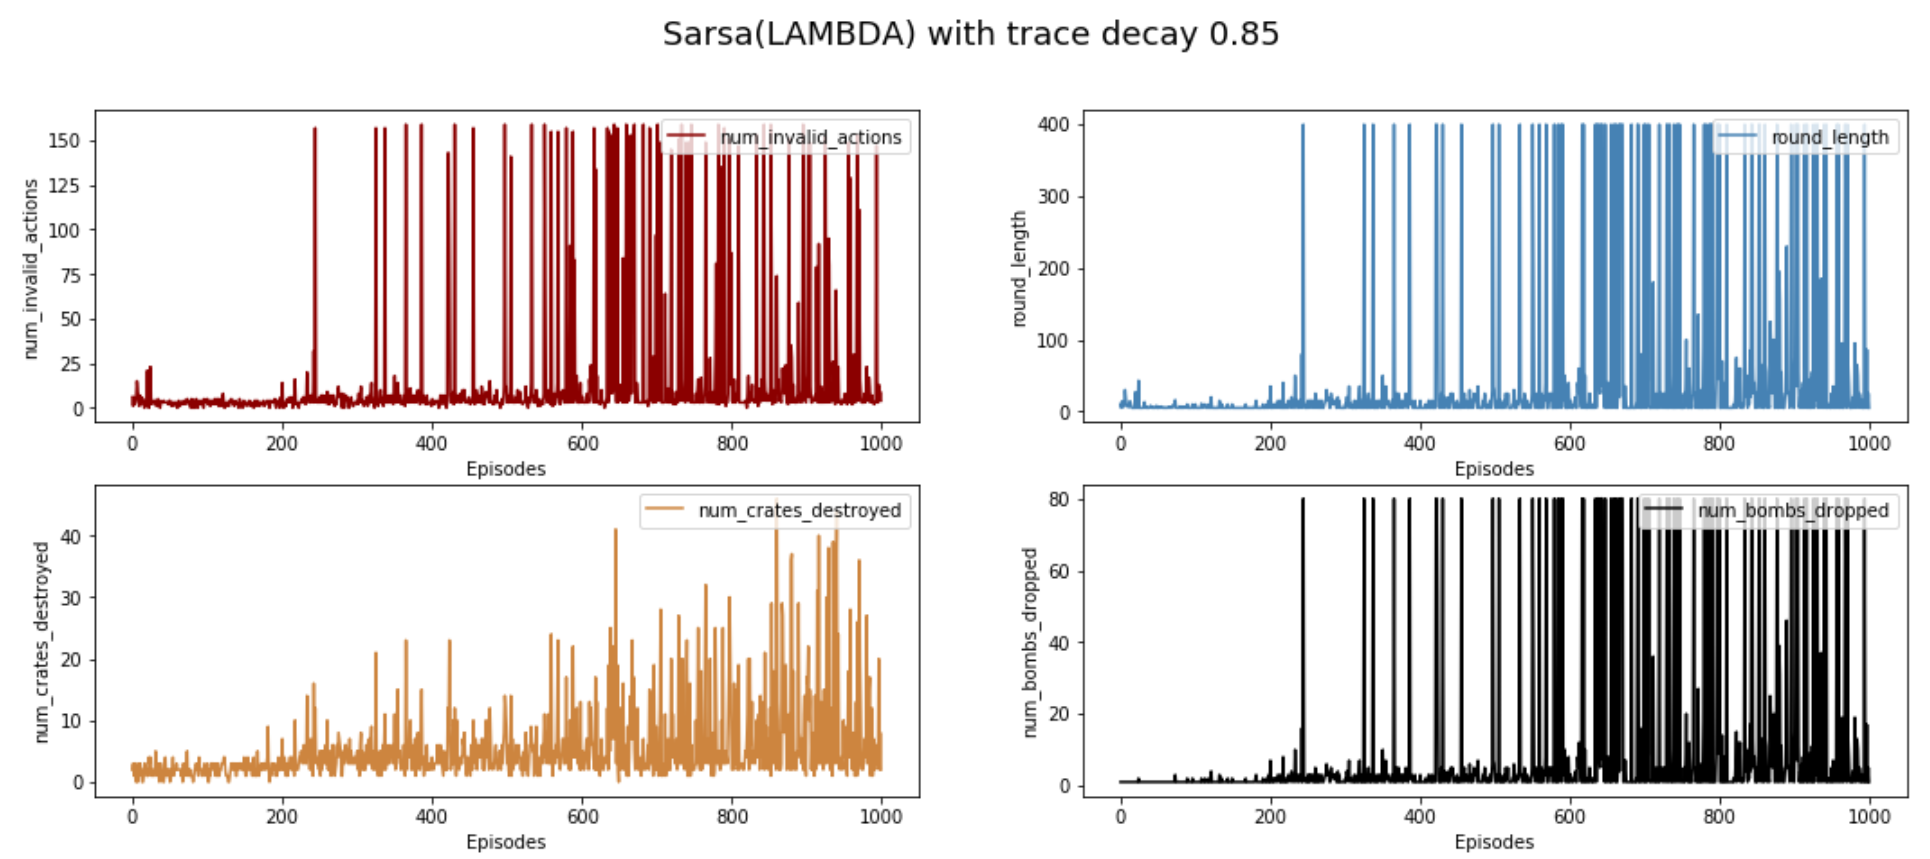
\includegraphics[scale=0.22]{graphics/plot05.png}
\end{center}
\begin{enumerate}
\setcounter{enumi}{1}
\item Never dropping a bomb was good. We used the same rewards as before but no rewards for dropping bombs. Everytime he dropped bombs he did not manage to escape, so he died directly. Leading to thinking that dropping them is bad.
\end{enumerate}
After this upsetting experience we created a custom event for giving the agent only a reward for setting a bomb at a position where he did not commit suicide. This also did not help directly since he would place the bombs at the right position but then die and get a good reward anyway.
\begin{center}
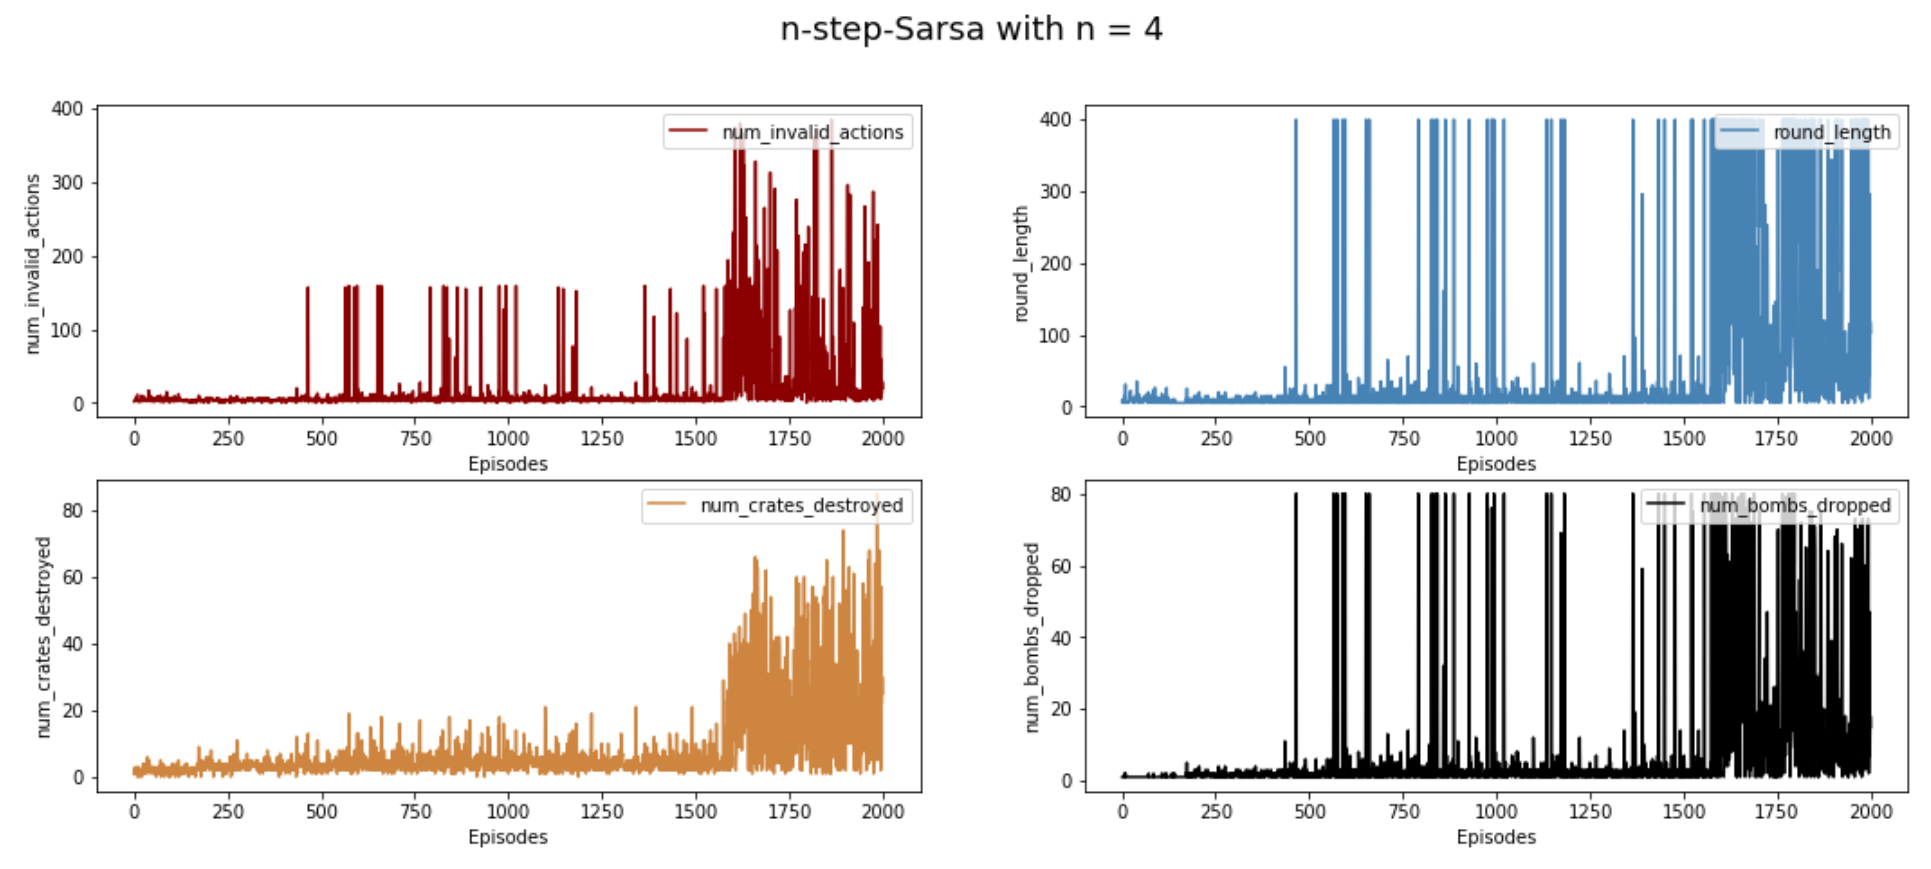
\includegraphics[scale=0.22]{graphics/plot06.png}
\end{center}

\section[Simulation study]{Simulation study \hfill \small \normalfont\textit{by Alessandro Motta}}

\subsection{Goals of the simulation study}
Thanks to our simulation study function we were able to make a comparison between $n$-step Sarsa and trace-decay for our linear agent. The parameters and the methods that we wanted to compare:
\begin{enumerate}
\item The $n$ for the $n$-step-Sarsa method
\item The $\lambda$ for the Sarsa($\lambda$) method
\item The learning rate ($\alpha$) 
\item The two methods with the different settings
\end{enumerate}

\subsubsection*{$\alpha$-comparison \& $n$ comparison}
All the graphs of the simulation study are in the file \texttt{simulation\_study.py}. The thing that helped us out the most of the simulation study was the learning-rate ($\alpha$) comparison. We had been using a learning rate that was too low. We could use a higher learning rate to get faster results.
\begin{center}
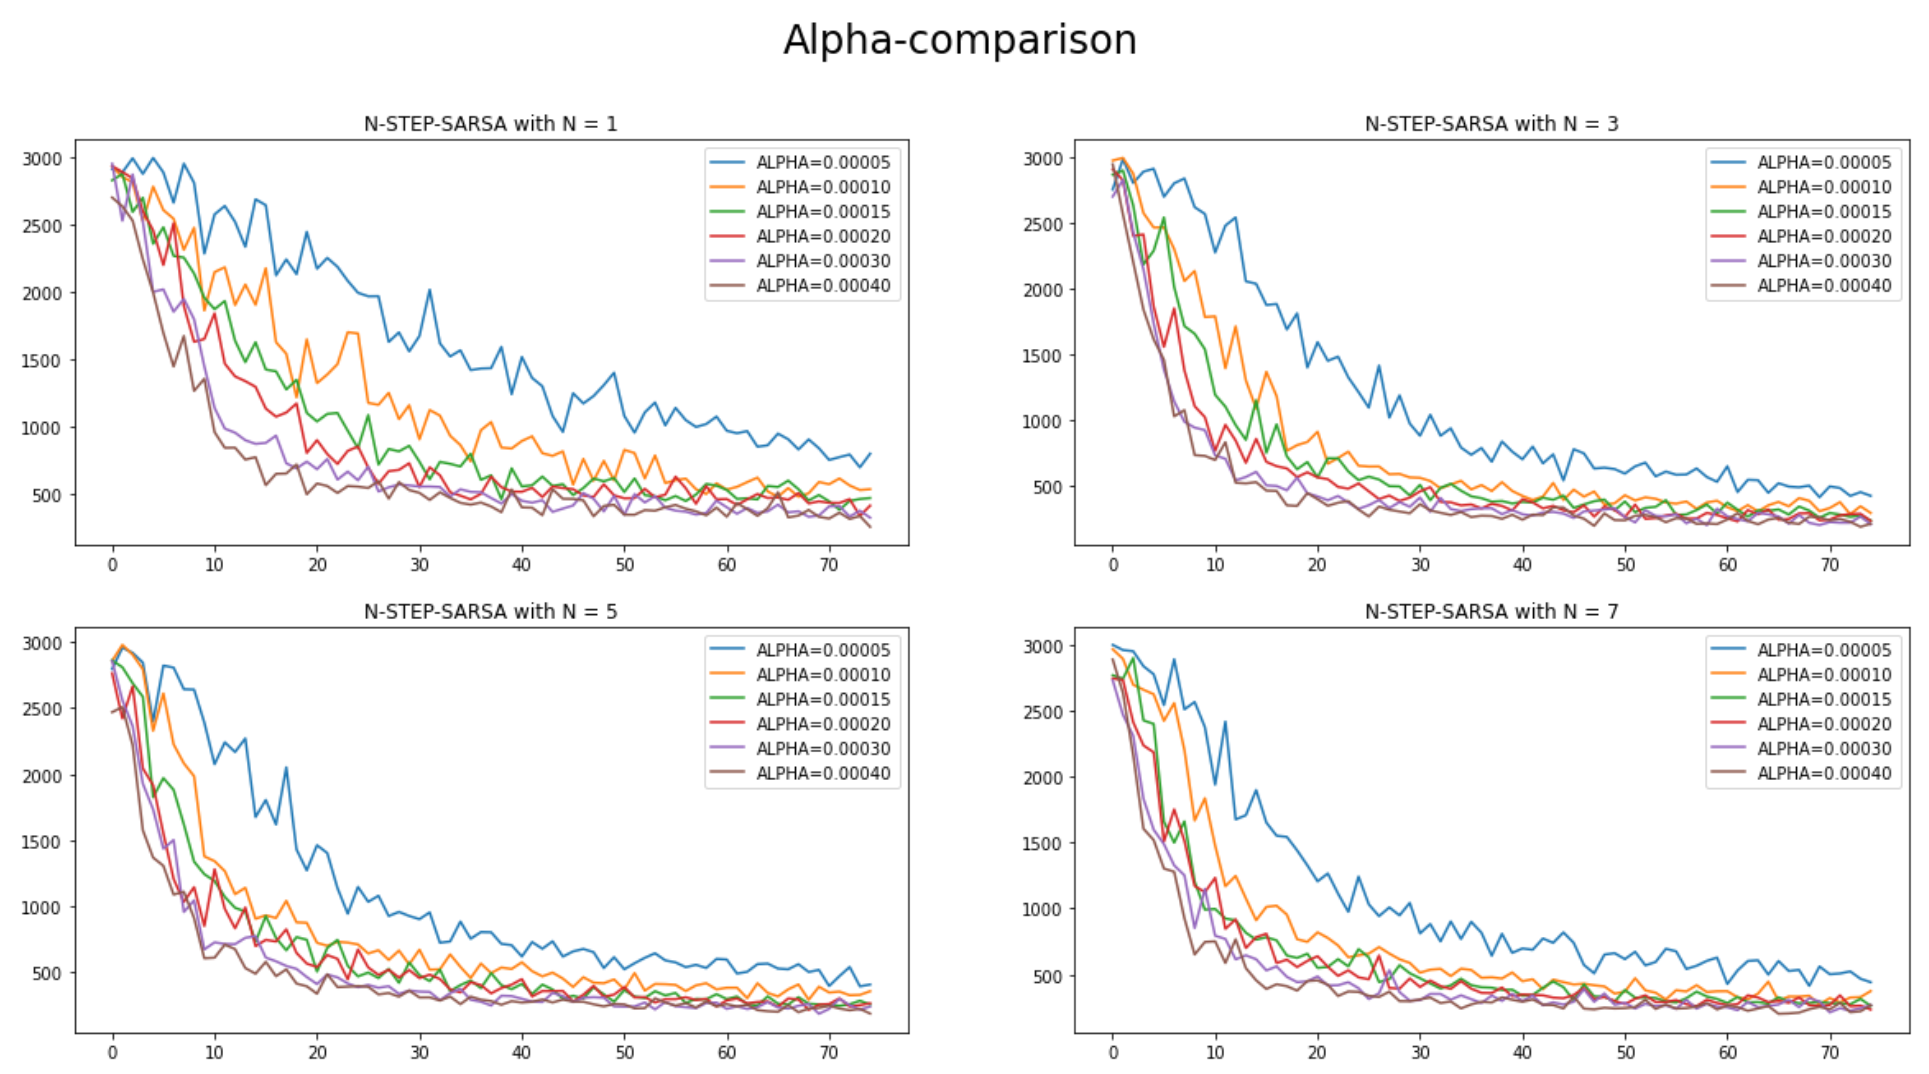
\includegraphics[scale=0.22]{graphics/plot07.png}
\end{center}
We chose this graph since the difference of how the learnig-rate can affect the training is really easy to see. On the $x$ axis we can observe the number of Episodes on the $y$ axis the number of the steps the game lasted. We used the coin collector agent (without shortest path) to make this study since we were already sure of its behavior and knew that it can converge. This means that to know how good the agent is we want to see that the episodes last less. Due to the fact that after collecting all the coins the episode was over. In the light blue we can see the smallest $\alpha$ value. It is observable that a bigger $\alpha$ leads to better results faster (see the brown or purple line for example). From this graph we could also deduct that using a $n>1$ for the $n$-step Sarsa method was better. We also made a $n$-comparison for $n$-step-Sarsa to be sure of this.
\\

We did the same thing for the Sarsa($\lambda$) method but noticed only a big difference between the different alpha values but not for the $\lambda$ values.
\begin{center}
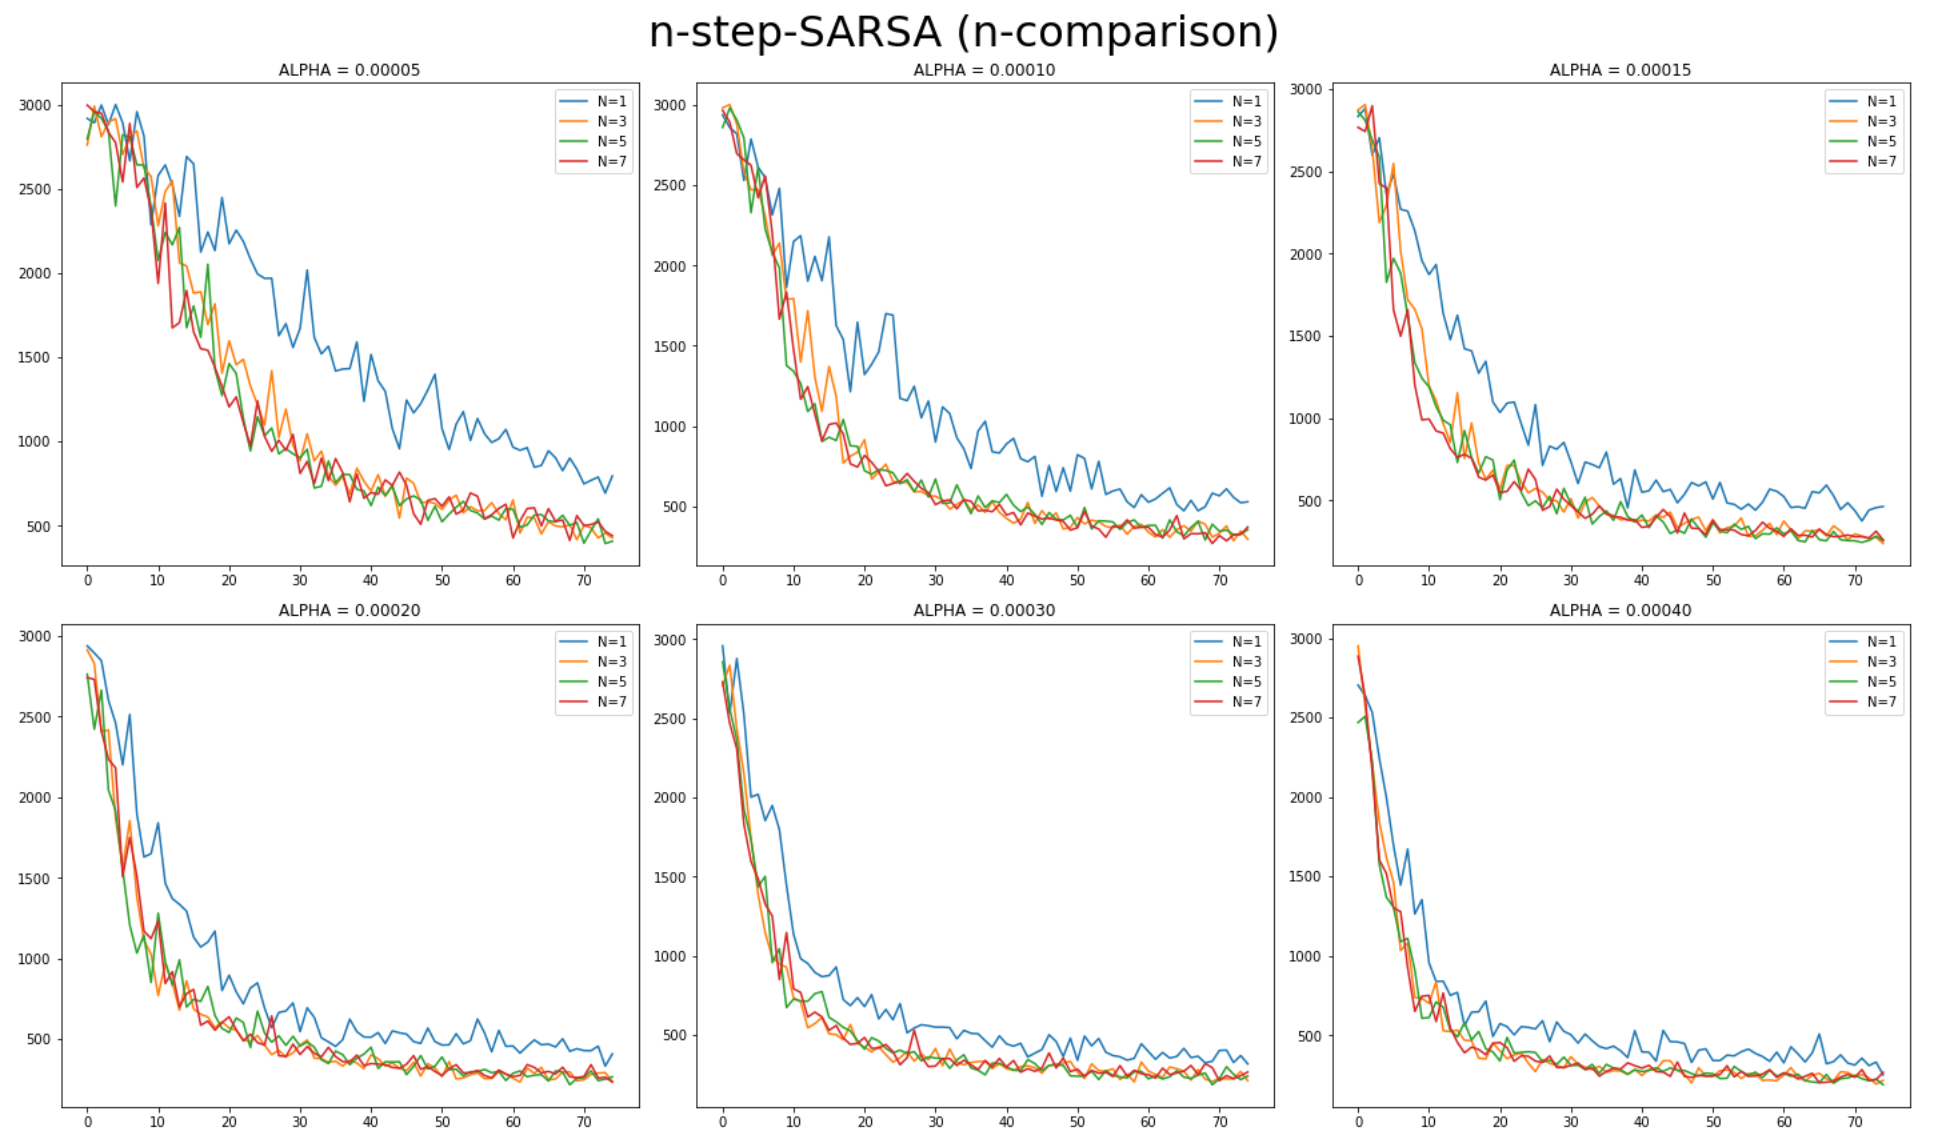
\includegraphics[scale=0.22]{graphics/plot08.png}
\end{center}

\subsubsection*{$n$-step Sarsa vs Sarsa($\lambda$)}
Last but not least we wanned to compare the two methods with each other. For this we took inspiration from a graph that we saw in the book \cite{Sutton1998} and plotted a similar graph. On the $x$-axis we can see the mean of the round length for the first 50 episodes and on the $y$-axis the different alphas. Note:
\begin{enumerate}
\item The graph depends also on the number of features that are used. For this plot we used 166 features. 
\item If we would have used a bigger $\alpha$ we might have seen how the lines would have started to go up (not learning as fast as our current $\alpha$'s).
\end{enumerate}
\begin{center}
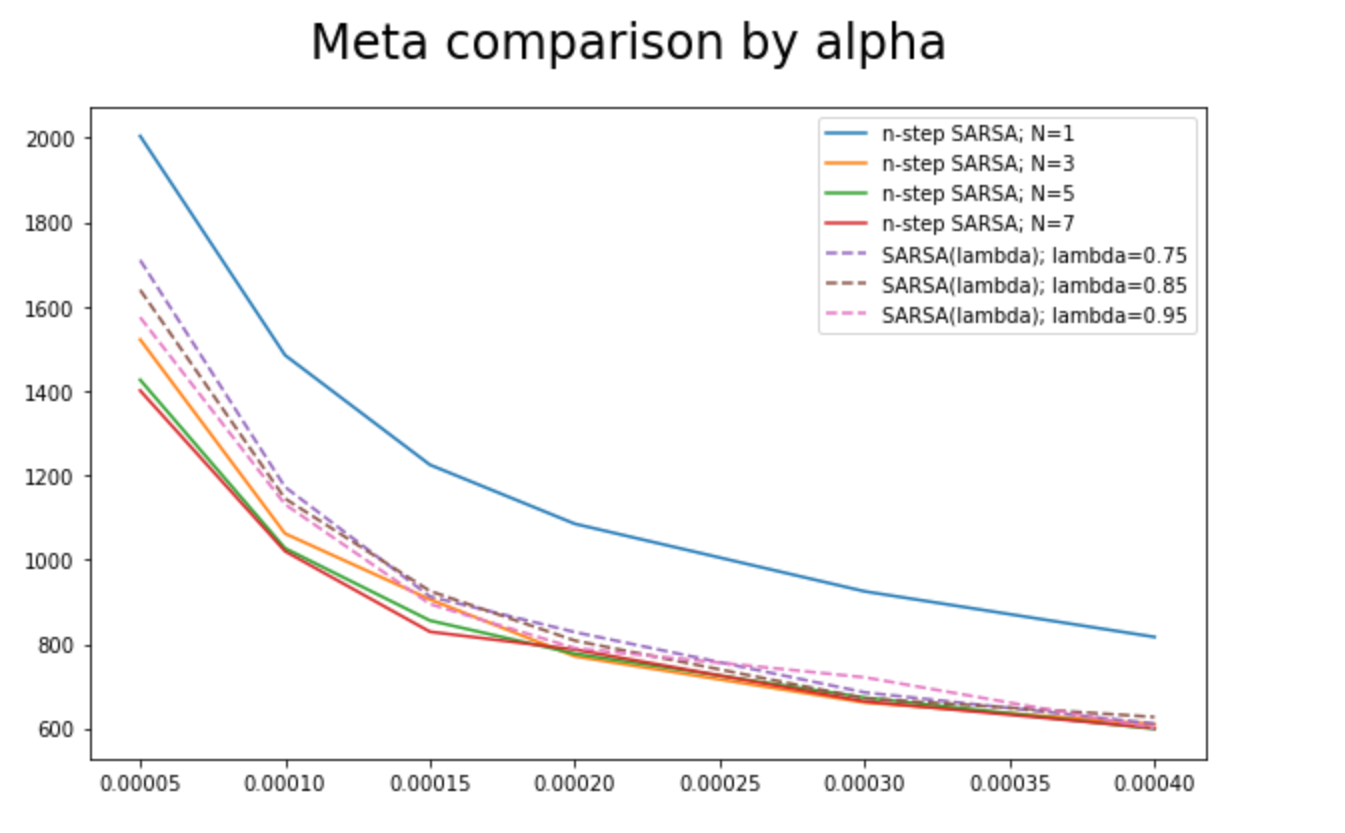
\includegraphics[scale=0.22]{graphics/plot09.png}
\end{center}


